\section{Computer Vision}

Computer vision attempts to solve the problem of replicating the functionality of human vision with a machine, specifically the extraction of useful information from images. This is a difficult problem to solve however, as in any given image we are supplied with insufficient information to fully specify as solution. Computer vision attempts to compensate for this lack of information by using physical and probabilistic models to produce high fidelity results. Advancements in computing power and access to larger and larger data sets has seen computer vision increasingly become a potential solution to old problems \cite{alg_apps}. There are many different techniques and areas of study within the field of computer vision and this section of the report outlines but a small fraction of them relevant to the subject matter of this report.  

\section{Contour Tracing}

Contour tracing also known as boundary tracing or border following is a method of locating images in a binary image by tracing their perimeter. It does so by generating a list of coordinates that comprise the outline of a connected-component of 1-pixels. 

The specific algorithm utilized in this system works was designed by Satoshi Suzuki in 1985 \cite{satoshi_findContours}. The algorithm works by identifying that a pixel is the edge of an object, determining if the border belongs to a hole or is the outer border of an object and labelling it accordingly. An important notation when considering this algorithm is that of 4- (8-) connectedness of a 1-pixel. A 4-connected pixel is a neighbour to every one of the pixels that touches it edges and an 8-connected pixel is a neighbour to every pixel that touches it edges and corners. Connectedness is used to determine if a pixel is part of a connected-component. Figure \ref{fig:connectedness} illustrates what these connections look like and Figure \ref{fig:connection_examples} illustrates some examples of 1-pixel connected-components and how they're connected.

\begin{figure}[H]
    \centering
    \centering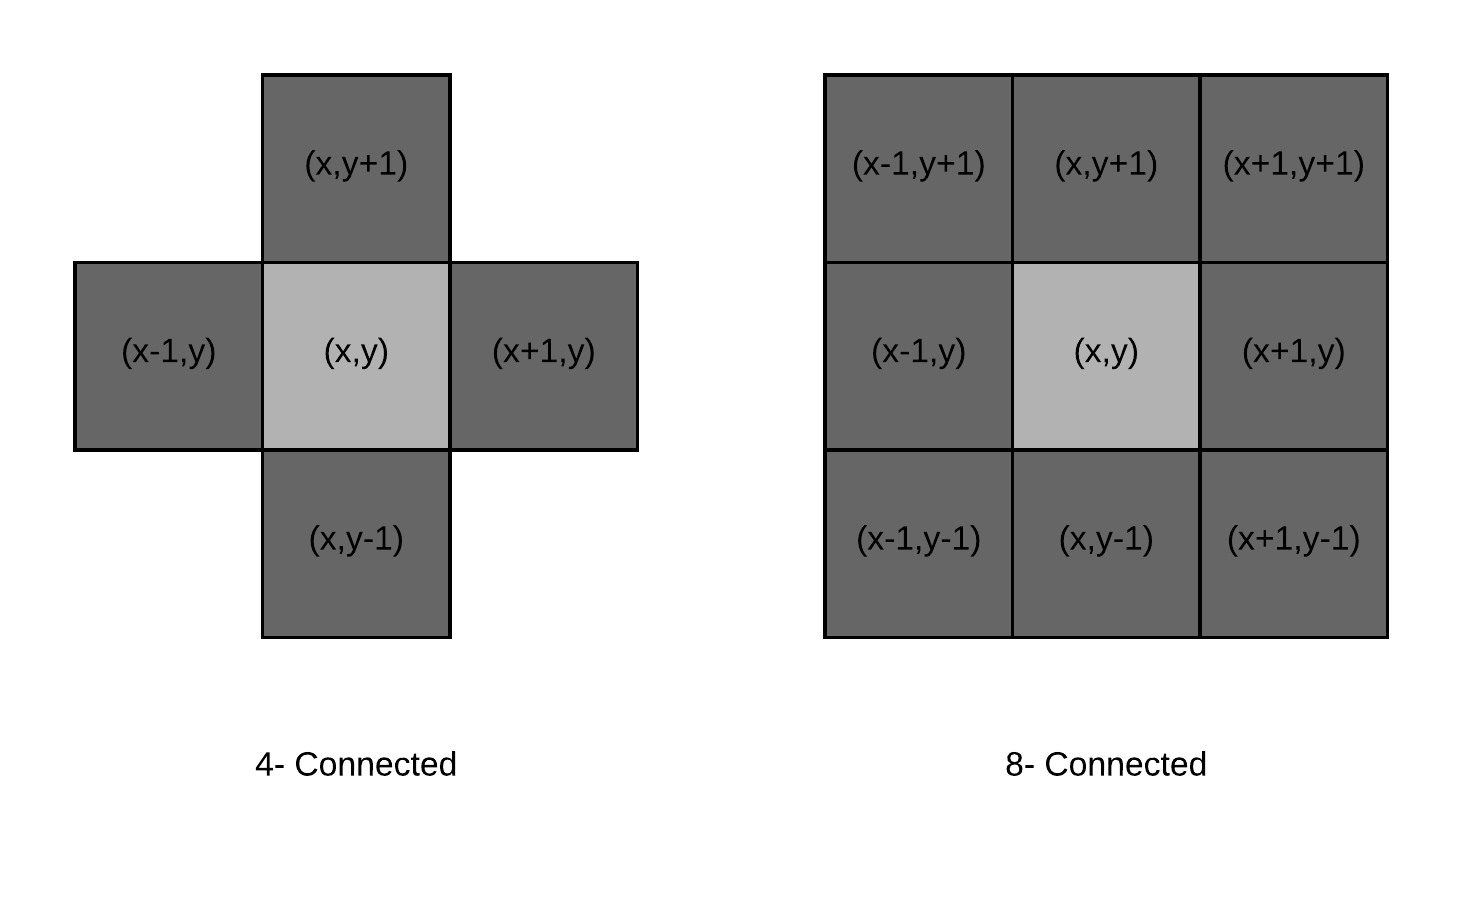
\includegraphics[width = 0.8\textwidth]{litreview/contours/connectedness.png}
    \caption{4- (8-) Connectedness of a pixel (x,y)}
    \label{fig:connectedness}
  \end{figure}

  \begin{figure}[H]
    \centering
    \centering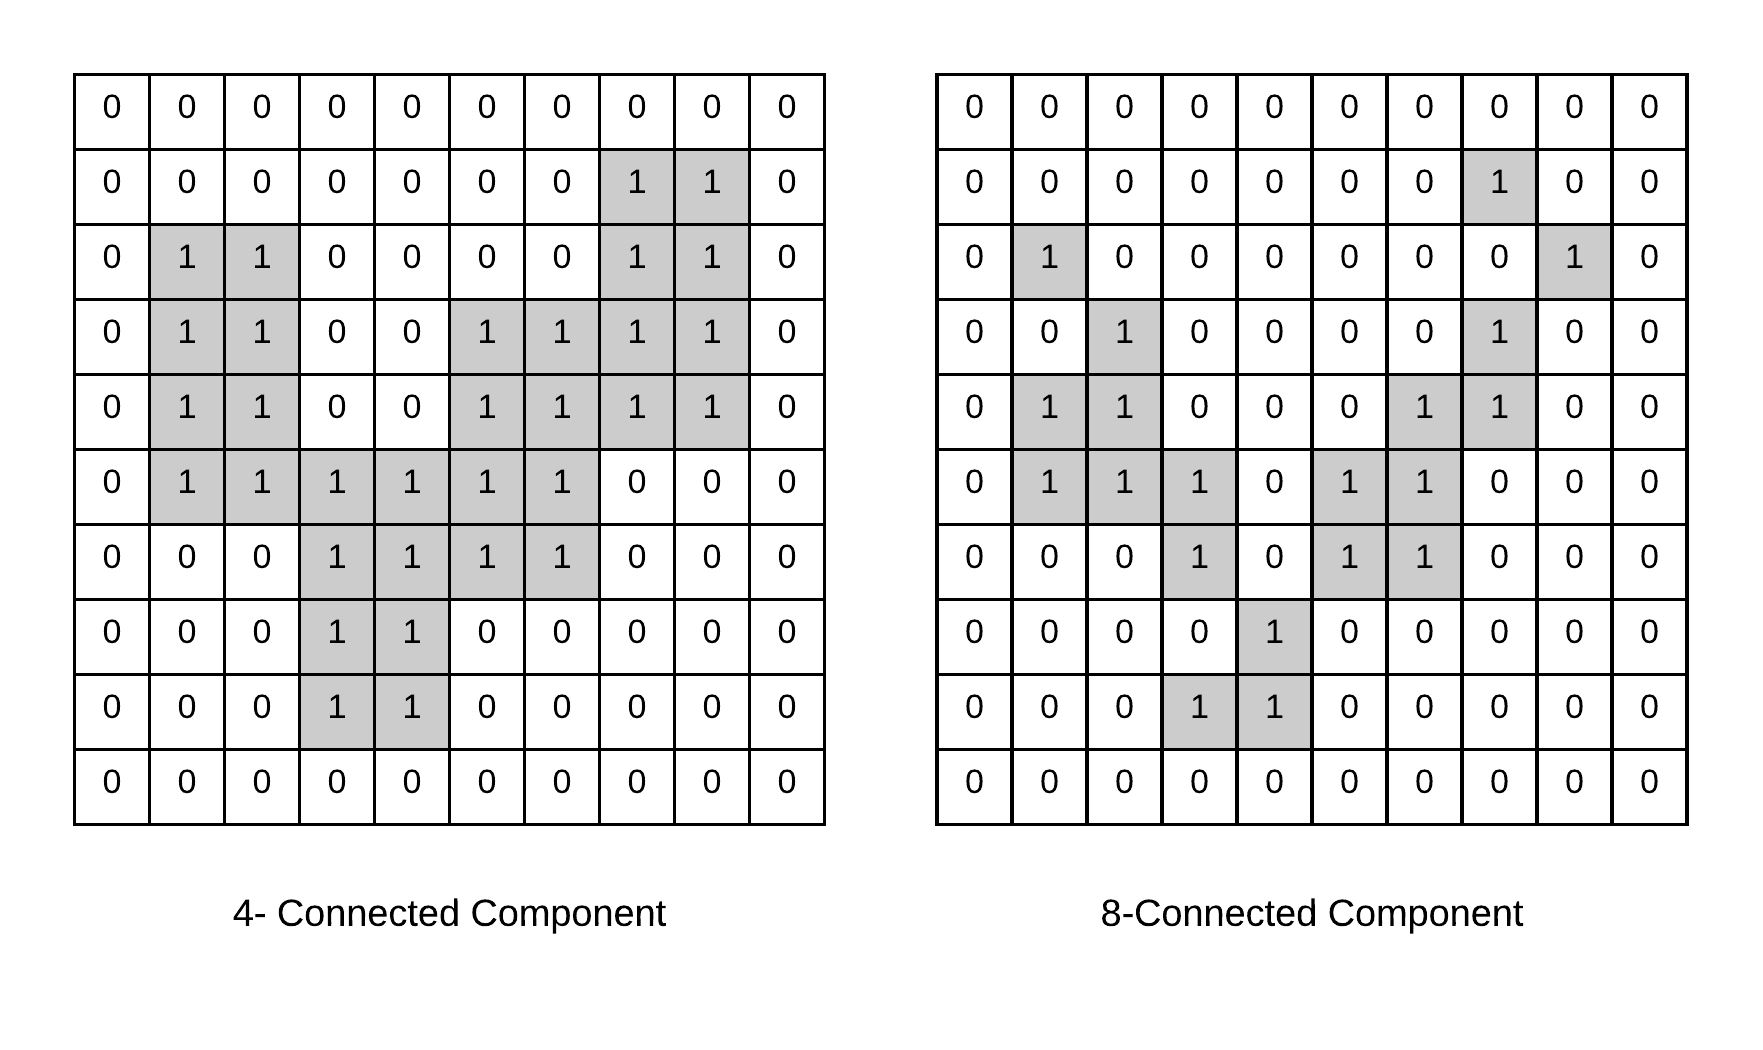
\includegraphics[width = 0.8\textwidth]{litreview/contours/connection_examples}
    \caption{Examples of different types of connected components.}
    \label{fig:connection_examples}
  \end{figure}
  

When the algorithm is performed the cells of the image are scanned in a raster fashion (left to right, top to bottom) and when a 1-pixel is encountered the algorithm interrupts and determines the type of border the pixel is that it ran into to. There are two types of border a hole border and an outer border. Figure \ref{fig:borders} illustrates these two types of borders. Satoshi defines a border point to be one that has a 0-pixel in its 4- (8-) neighborhood. An outer border is one surrounded by 0-pixel connected component and a hole border is one that surrounds a 0-pixel component. If a border is has thickness of only one pixel and is satisfies both being an outer border and hole border it's regarded as an outer border. The high-level outline of the algorithm is specified in Algorithm \ref{algorithm:satoshi} though the source material \cite{satoshi_findContours} should be consulted for a more comprehensive description.

\begin{figure}[H]
    \centering
    \centering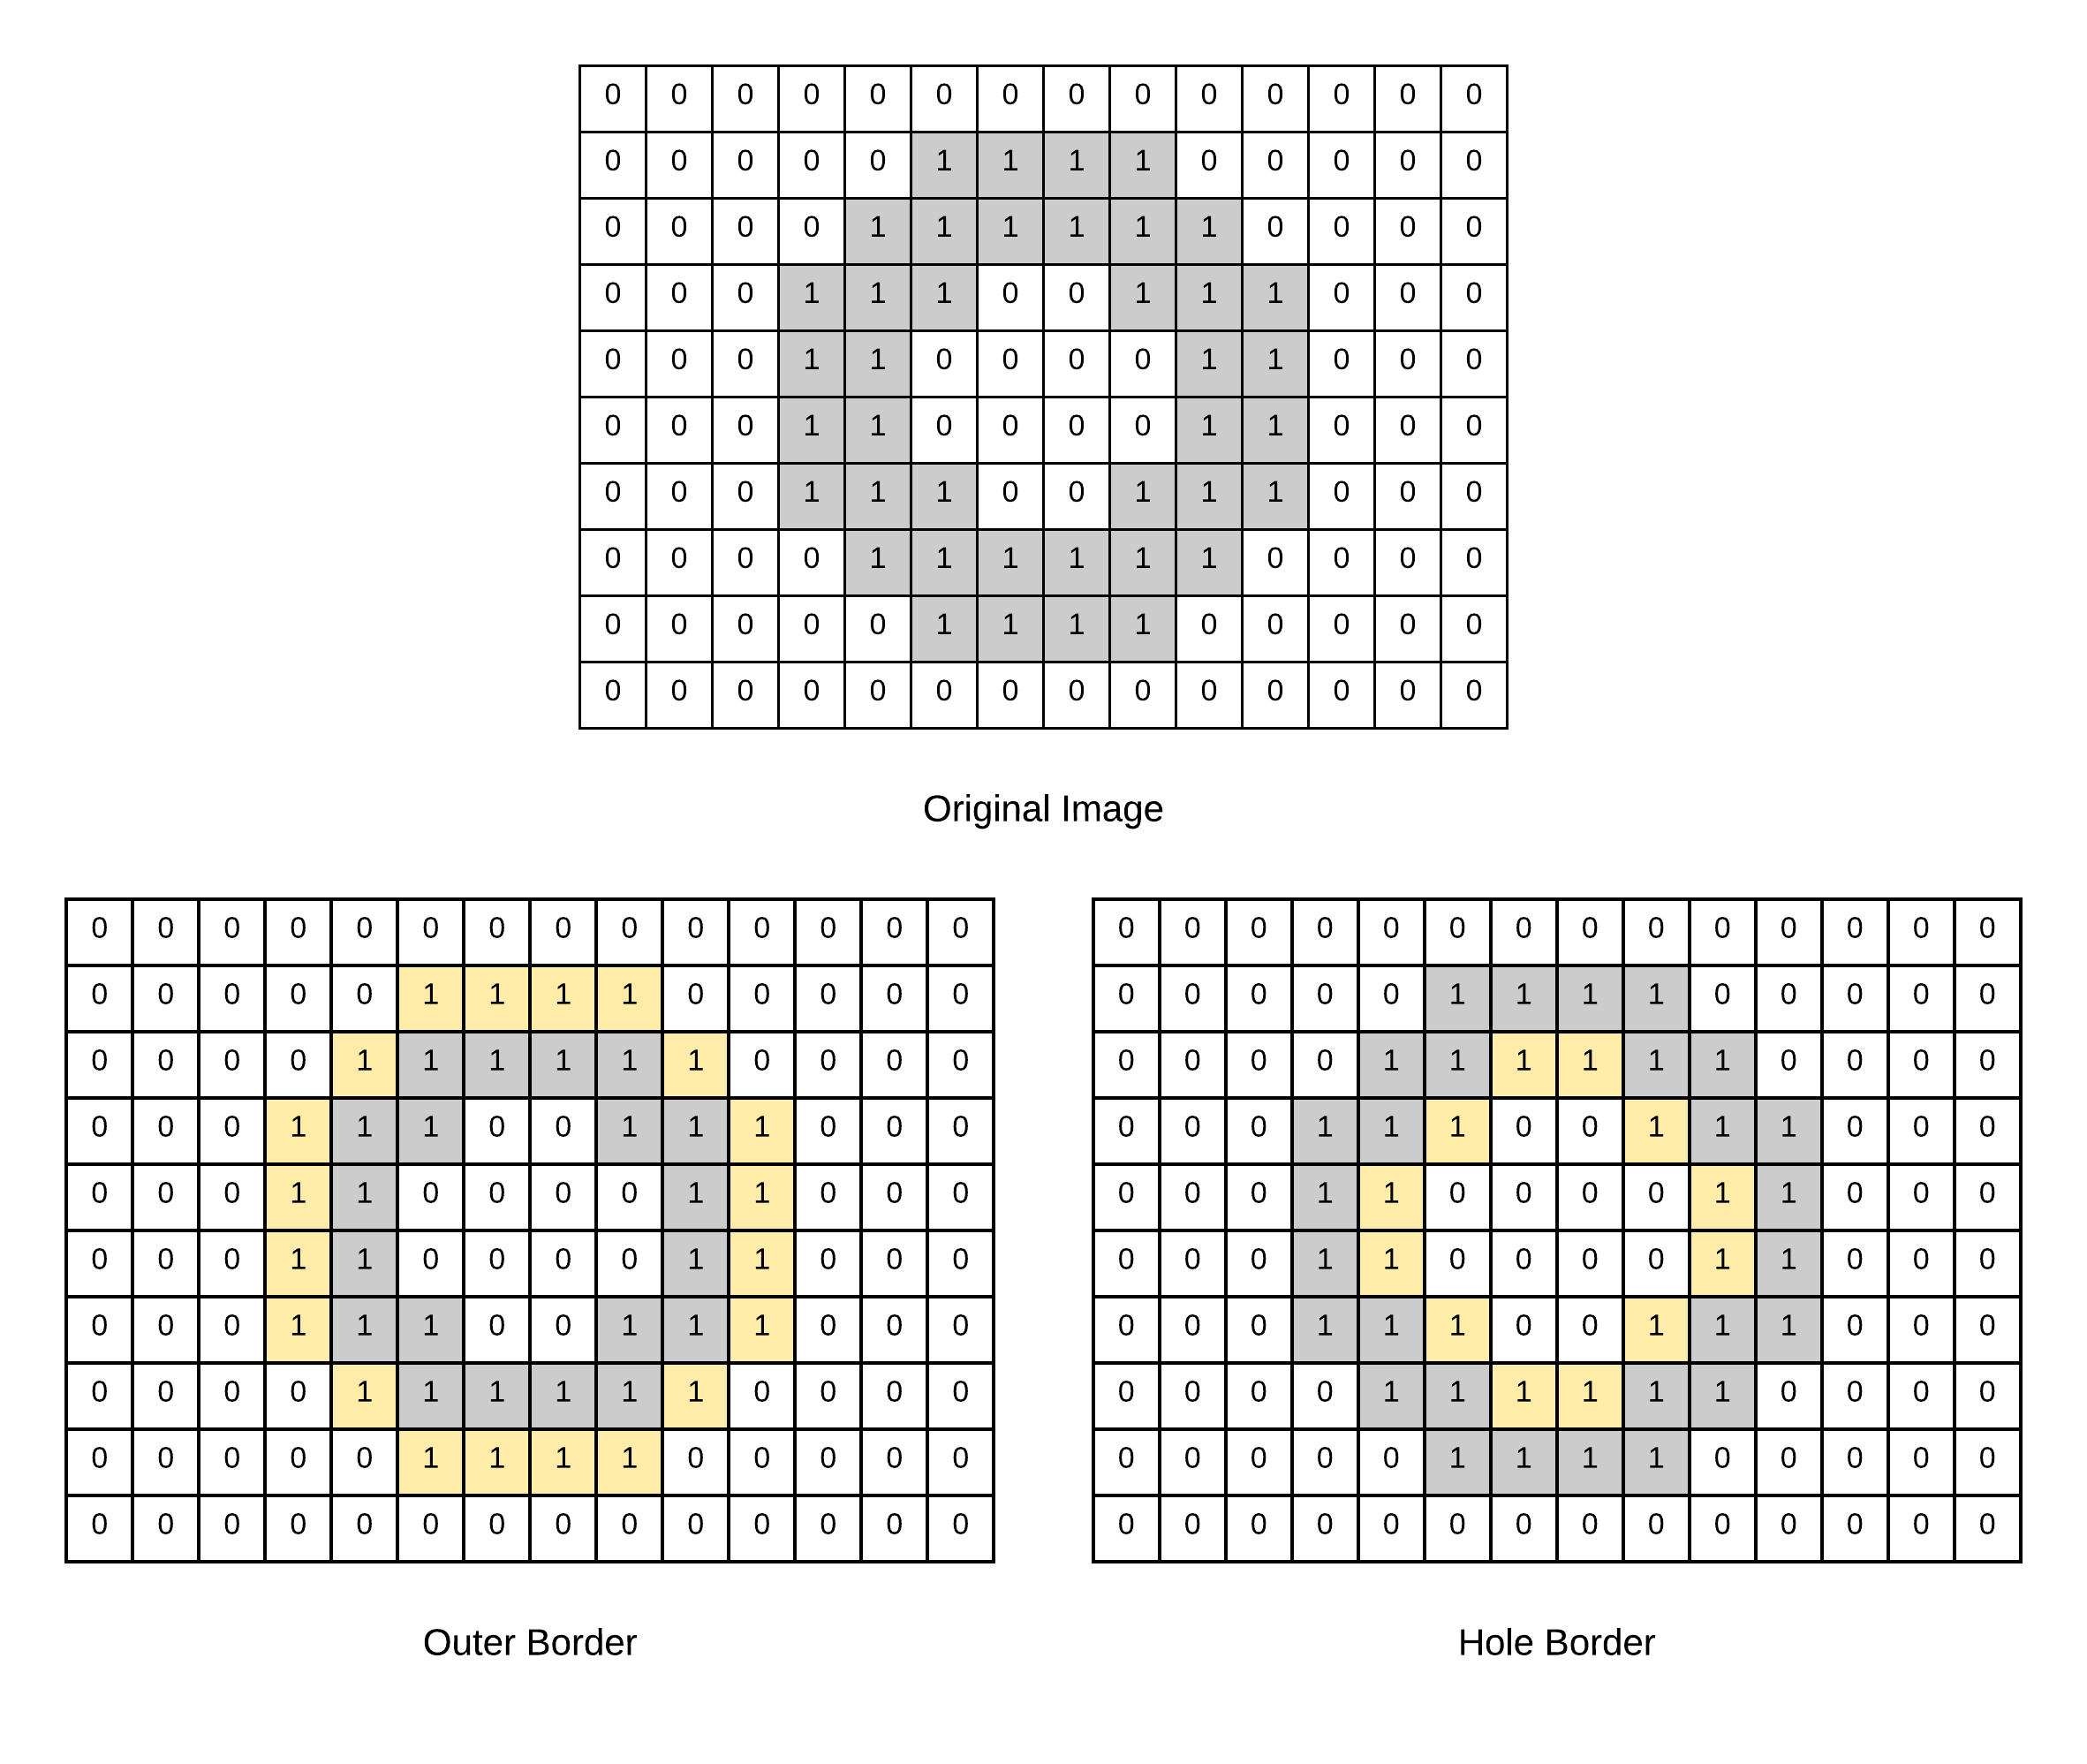
\includegraphics[width = 0.8\textwidth]{litreview/contours/borders}
    \caption{Comparison of a hole border and outer border.}
    \label{fig:borders}
  \end{figure}


\begin{algorithm}
\SetAlgoLined
\KwInput{Binary image, F, size I x J} 
\KwOutput{Coordinates of all object borders in F}
Initialize LNBM = 1 which tracks most recently labelled border.\;
Initialize counter NBD = 0 which tracks the number of borders created.\;
\While{imageScanner $\neq$ F[I,J]}{
    \uIf{F[i,j] = 1 and F[i,j-1] = 0}{
        F[i,j] is the starting point of an outer border\;
        follow border until return to starting point labelling all points with a unique ID\;
    }\uElseIf{F[i,j] $\geq$ 1 and F[i,j+1] = 0}{
        F[i,j] is the starting point of a hole border\;
        follow border until return to starting point labelling all points with a unique ID\;
    }
}
\caption{Satoshi Suzuki's algorithm for border tracing \cite{satoshi_findContours}.}
\label{algorithm:satoshi}
\end{algorithm}


  


\subsection{Tracking}

The tracking component of the detection algorithm takes a list of bounding box coordinates corresponding to each foreground object and generates tracked objects that contain the coordinates history of the objects. 

Each vehicle object's location in an image is represented by the centre of its bounding box, called a centroid, by maintaining a history of an object's centroid position over time its path can be tracked through the video. For each image new centroids are recalculated for every object and by comparing the new centroid locations with the old centroid locations the new position of objects can be determined. New centroids are assigned to the objects whose last known position was closest. Algorithm \ref{algorithm:centroid_reassign} outlines the centroid reassignment process.

\begin{algorithm}
  \SetAlgoLined
  \KwInput{List of current centroids \emph{cen\_old}, size X, List of new centroids \emph{cen\_new}, size Y} 
  \KwOutput{Updated list of current centroids}
  Generate an $X \times Y$ distance matrix, $D$, between \emph{cen\_old} and \emph{cen\_new}\;
  Generate a list of column indices, \emph{cols} from $D$ sorted by the column containing the smallest value to the largest\;
  Generate a list of row indices, \emph{rows}, from $D$ corresponding to the row containing the smallest values in \emph{cols}.\;
  \For{(i,j) in (\emph{rows}, \emph{cols})}{
    \If{cen\_new[j] not used and cen\_old[i] not used}{
        \emph{cen\_old[i]} = \emph{cen\_new[j]}\;
        mark \emph{cen\_old[i]} as used\;
        mark \emph{cen\_new[j]} as used\;
    }
  }
  \For{\emph{cen} in unused \emph{cen\_new}}{
    \emph{cen\_old}.append(\emph{cen})\;
  }
  \For{\emph{cen} in unused \emph{cen\_old}}{
    mark \emph{cen} as missing\;
  }
  \caption{Centroid re-assignment algorithm. \cite{adrian_rosebrock_simple_object_tracking}}
  \label{algorithm:centroid_reassign}
\end{algorithm}

If a new position cannot be found for an object then it has a limited number of frames it can be missing for before it's removed, objects generally go missing due to partial or complete occlusion by other vehicles, alternatively they will go missing permanently if they leave the node's field of view. Vehicle's can also disappear if they remain stationery long enough to be considered background pixels by the subtractor. Figure \ref{fig:centroids} visualizes the centroids on the objects along with a unique identifier which is used to mark ownership of a foreground object. Notice in Figure \ref{fig:centroids} centroids 25 and 24 belong to no object, this is because they have not yet timed out, meaning their object hasn't been missing from frame long enough for them to be dismissed, this is also the case for centroid 16. Centroids 1 and 9 belong to a cluster of vehicles that have become distant (see Figure \ref{fig:original_frame}), this occurs because as the vehicles travel further away the distance between them in pixels becomes less and so the morphological process presses them together. This is not an issue if the counting and measuring system is calibrated to focus on areas where vehicles are easily separable. 

\begin{figure}[H]
    \centering
    \centering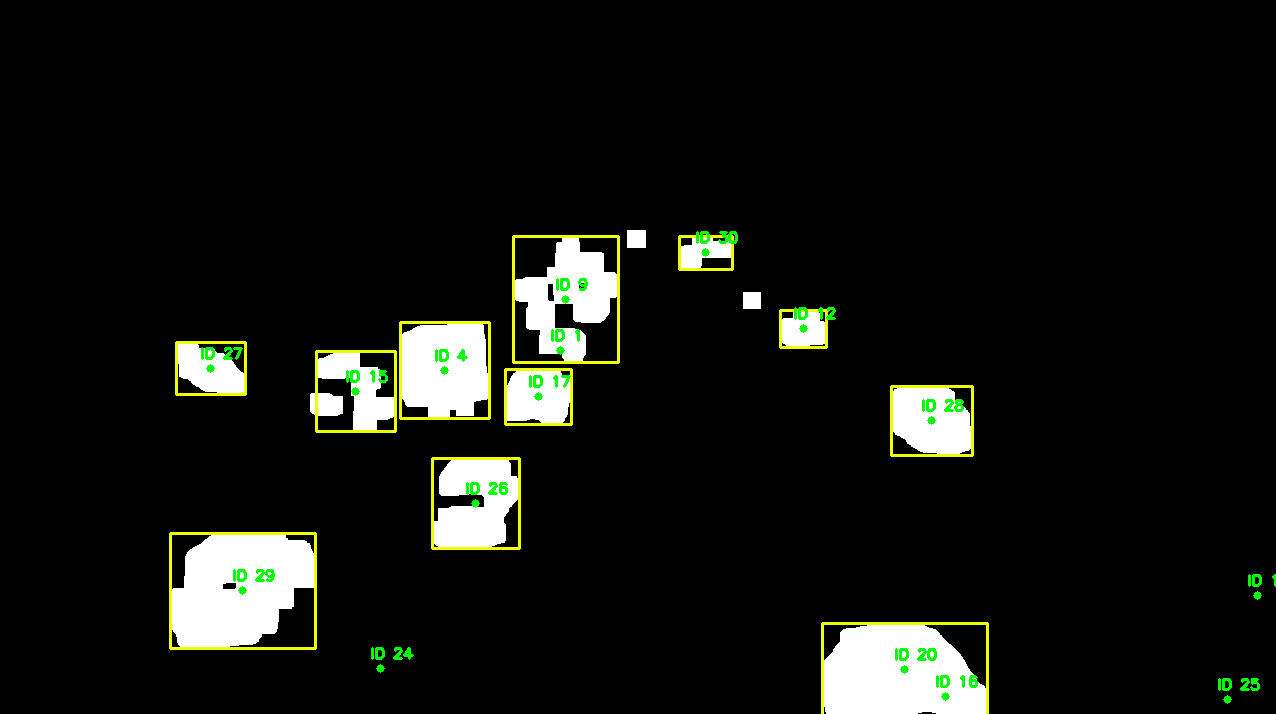
\includegraphics[width = 0.8\textwidth]{design/detection/tracking/mask_centroids}
    \caption{Centroids plotted over foreground objects.}
    \label{fig:centroids}
\end{figure}

\subsubsection{Calibration}

For a given traffic scenario we seek to set a maximum\_distance and minimum\_distance which control centroid reassignment. We also should consider the amount of time a object can go missing for. 

The minimum\_distance parameter addresses failure of the morphology component of the algorithm to recombine some blobs. After all centroids are reassigned an additional consolidation process is performed where if any two centroids are closer together than min\_distance they are merged into a single centroid. Figure \ref{fig:centroids_consolidation} compares two centroid allocations for the same image where one performs centroid combination and the other doesn't. In Figure \ref{fig:consolidateA} the number of centroids is greater thus consuming more computational power and increasing the number of false positive counts.

Maximum\_distance controls the allowed distance a new centroid can be from an old one and still be considered its new position. In cases where there are more new centroids than old ones, without this parameter restriction, centroid allocations will store an old centroid's an unreasonable distance from its old position when in reality a new centroid should be generated and not reassignment performed.

The second calibration consideration for tracking is how long the system allows an object to be missing. Determination of this quantity dependent on how frequently vehicles are occluded and for how long. In a situation where there was an obstacle consistently blocking vision of the road for a period then the amount of time a centroid should be stored is proportional to how long a vehicle is occluded by that obstacle on average. Its common that an object may disappear for a few frames so it's important for objects to be able to go missing and remerge else lots of data could be lost.

\begin{figure}[H]
\centering
\begin{subfigure}[b]{0.45\linewidth}
            \centering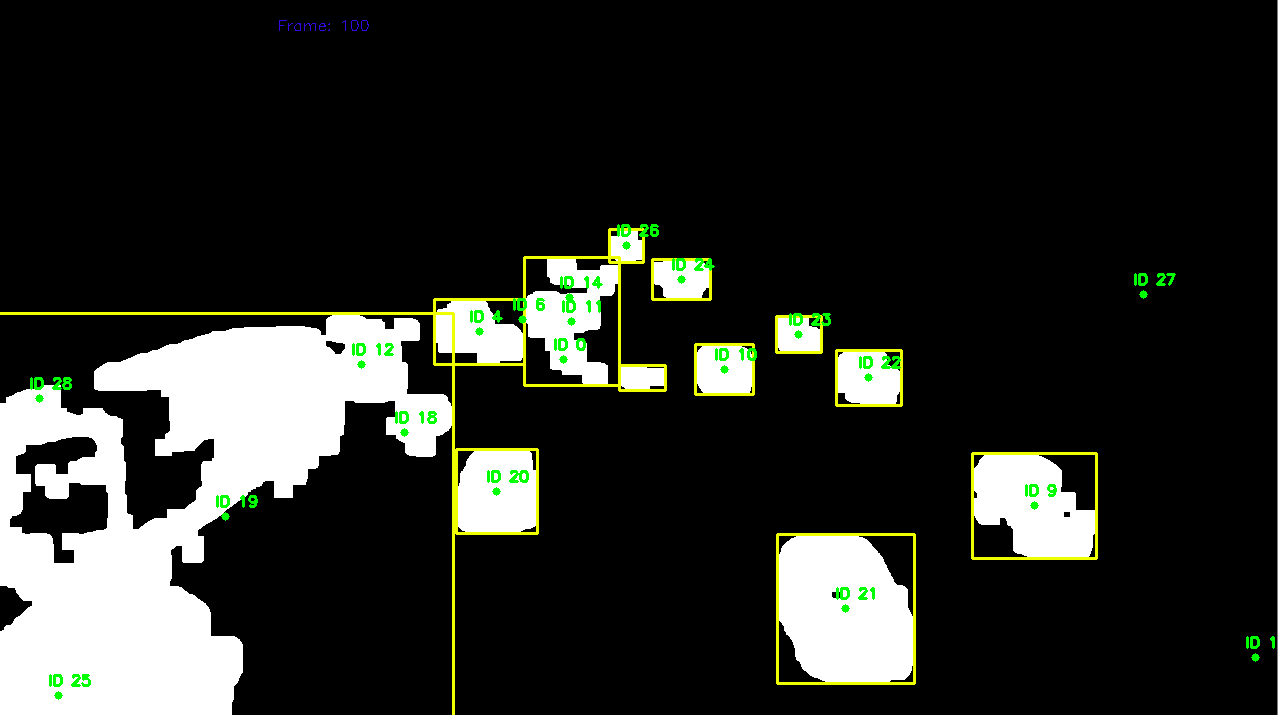
\includegraphics[width = \textwidth]{design/detection/calibration/mask_noconsolidate}
            \captionsetup{format=hang}
            \caption{Centroid tracking with no consolidation distance set (16 centroids).}
            \label{fig:consolidateA}
  \label{fig:}
    \end{subfigure}
    \begin{subfigure}[b]{0.45\linewidth}
            \centering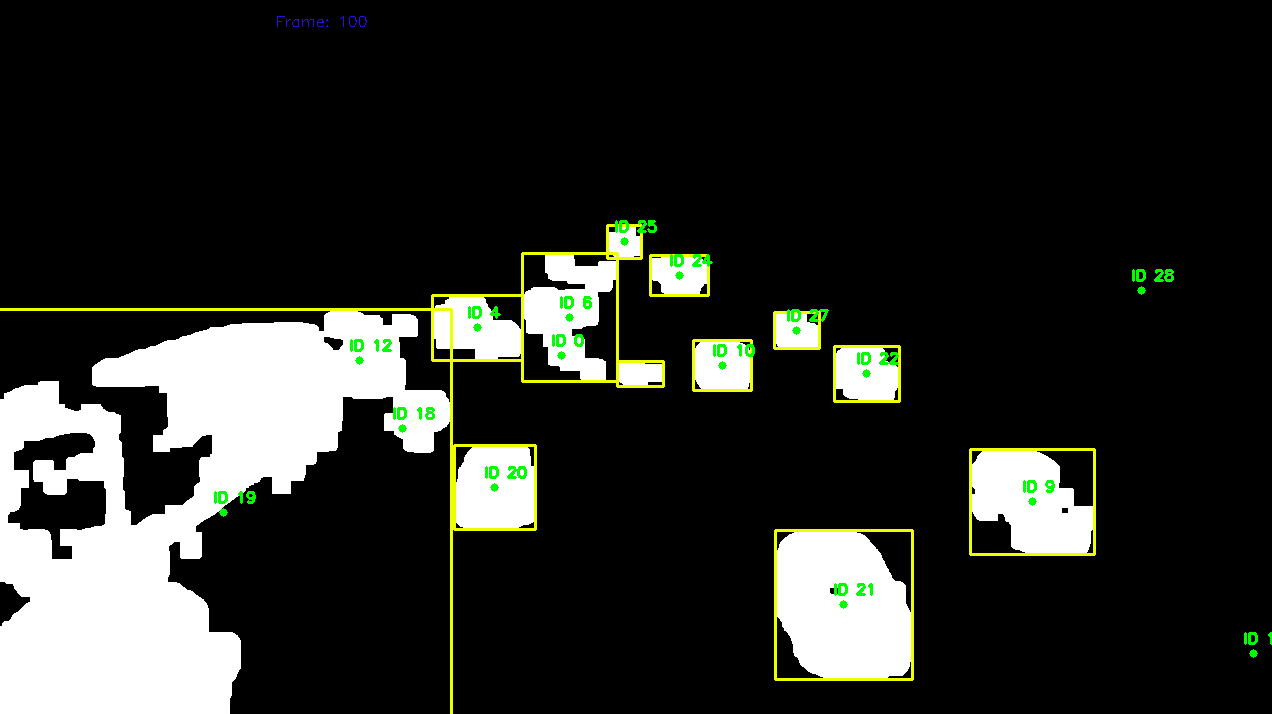
\includegraphics[width = \textwidth]{design/detection/calibration/mask_consolidate}
            \captionsetup{format=hang}
        \caption{Centroid tracking with consolidation distance set (20 centroids).}
        \label{fig:consolidateB}
      \end{subfigure}
      \captionsetup{format=hang}
    \caption{Comparison of centroid generation with and without consolidating centroids based on distance.}
    \label{fig:centroids_consolidation}
\end{figure}
  


